\documentclass{article}
\usepackage{graphicx}
\usepackage[utf8]{inputenc}
\usepackage{amsmath, amssymb, latexsym}
\usepackage{neuralnetwork}
\usepackage{multicol}
\usepackage{expl3}

\usepackage{pgfplots}
\usepackage{algorithm}
\usepackage[noend]{algpseudocode}
\usepackage{tikz}
\usepackage{nicefrac}
\pgfplotsset{every axis legend/.append style={
at={(0,0)},
anchor=north east}}
\usetikzlibrary{shapes,positioning,intersections,quotes}
\usetikzlibrary{arrows.meta,
                bending,
                intersections,
                quotes,
                shapes.geometric}
                
\definecolor{darkgreen}{rgb}{0.0, 0.6, 0.0}
\definecolor{darkred}{rgb}{0.7, 0.0, 0.0}
\makeatletter
\begin{document}

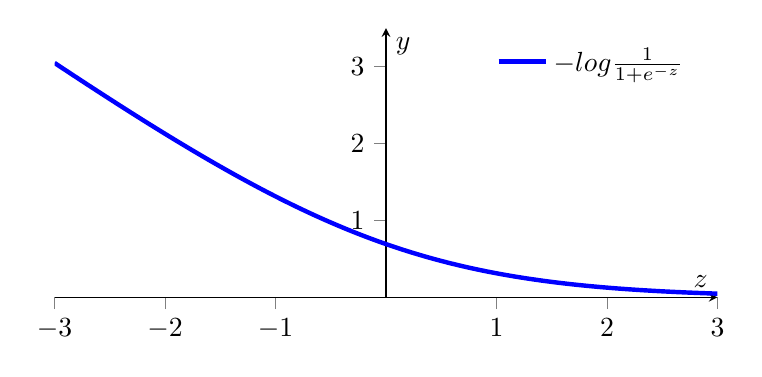
\begin{tikzpicture}
  \begin{axis}[
      axis x line=middle,
      axis y line=middle,
      width=10cm,
      height=5cm,
      xmin=-3,   % start the diagram at this x-coordinate
      xmax= 3,   % end   the diagram at this x-coordinate
      ymin=0,   % start the diagram at this y-coordinate
      ymax= 3.5,   % end   the diagram at this y-coordinate
      xlabel=$z$,
      ylabel=$y$,
      legend cell align=left,
      legend pos=north east,
      legend style={draw=none},
      tick align=outside,
      enlargelimits=false]
    % plot the function

    \addplot[domain=-3:3, blue, ultra thick,samples=500] {-ln(1/(1+exp(-x)))};
    \legend{$-log \frac{1}{1+e^{-z}}$}
  \end{axis}
\end{tikzpicture}


\end{document}
